%%%%%%%%% PROJECT DESCRIPTION  -- 10 pages (including Prior NSF Support)

\renewcommand{\P}{\textrm{Pr}}
\newcommand{\E}{\mathbb{E}}

%\renewcommand{\thefootnote}{\fnsymbol{footnote}}
%\makeatletter\stepcounter{\@mpfn}\makeatother

\newcommand{\ie}{\emph{i.~e.},\xspace}
\newcommand{\eg}{\emph{e.~g.},\xspace}
\newcommand{\etal}{\emph{et~al.}\xspace}
\newcommand{\sig}[1]{\ensuremath{\textrm{sig}(#1)}}

\newcommand{\atime}{\texttt{atime}\xspace}
\newcommand{\ctime}{\texttt{ctime}\xspace}
\newcommand{\MWs}{\textit{Model workloads}\xspace}
\newcommand{\MW}{\textit{Model workload}\xspace}
\newcommand{\mWs}{\textit{model workloads}\xspace}
\newcommand{\mW}{\textit{model workload}\xspace}

\newcommand{\Mws}{Model workloads\xspace}
\newcommand{\mws}{model workloads\xspace}
\newcommand{\mw}{model workload\xspace}
\newcommand{\Mw}{Model workload\xspace}

%\required{Project Description}
%
%All proposals to NSF are reviewed utilizing the two merit review criteria,
%intellectual merit and broader impacts. \\

% The Project Description should provide a clear statement of the work 
% to be undertaken and must include: objectives for the period of the proposed 
% work and expected significance; relation to longer-term goals of the PI's 
% project; and relation to the present state of knowledge in the field, 
% to work in progress by the PI under other support and to work in progress 
% elsewhere.

\section{Introduction}

%iiAs modern applications expand in complexity and scale, we compound the difficulty of %{{{
%%ensuring adequate performance for their users. 
%The software driving today's computers, cell phones and cars has grown to comprise tens of millions of lines of code \cite{informationisbeautiful},
%making it challenging to optimize the programs for speed.
% http://www.informationisbeautiful.net/visualizations/million-lines-of-code/
%Yet users continually demand for low-latency interactions and vote with their wallets.%}}}


%** WHAT IS THE PROBLEM?
%Storage systems research is the study of trade-offs between security,
%reliability, availability, and performance.  High impact projects highlight
%special cases in this tuning.

The overarching theme of this research project is
to improve system provisioning by developing a series of programs to identify important workload features (%FIXME NAME
)
, evaluate workload characteristics (%FIXME name
)
and apply this knowledge to different infrastructures (%FIXME name
) to address three costly pitfalls storage provisioning for current and rapidly evolving storage demands.\\ 


All storage systems exist to serve a group of users and applications with specific and often unique characteristics.
Tuning a storage system is a delicate
balance between reliability, availability, security, and performance spread over the
users, or workloads, that the system serves. 
 The technological (better word?) devices we use and continue to develop are not just networked, but
share huge volumes of data alongside instantaneous and sometimes vital decisions.
Technologies such as self-driving cars, smart cities and homes, and augmented
reality all depend on handling massive quantities of data quickly and reliably.
Understanding the characteristics of workloads such as these will be critical to both
reducing storage costs and making the cloud of tomorrow accessible and equitable
for all.

%Imagine too, a world where there are clouds everywhere; where the devices we use%{{{
%are not just networked, but share the burden of huge volumes of data and
%instantaneous decisions, where software is seamlessly managed across
%infrastructure wherever in the world it resides, and where these technologies
%are available as open source to any company.  
%
%That’s a truly exciting wave of innovation.

%AND THIS HIDDEN BIT SEEMS LIKE YOUR INTRO VISION STATEMENT FRIEND! Just make it less TED-talk intro and more possibly applicable. I think the part below might be part of a more concrete application of it. 
%%
%The advent of self-driving cars will force many changes in how computing and
%communications systems are architected, both through hardware and software. It’s
%these advances in data management, combined with edge computing that will enable
%driverless cars, smart cities and homes, and other connected technologies.
%]
%
%http://news.ihsmarkit.com/press-release/automotive/autonomous-vehicle-sales-set-reach-21-million-globally-2035-ihs-says%}}}


%There are many factors, from cache size to device type to the redundancy model, to balance when designing a storage system.
%, which together form a set of
%workloads that pass through the system.
  Over time the usage of systems is certain to shift as new hardware and
  software technologies  become available.
  For cloud storage, elasticity is a
crucial factor, but misconfiguration in reactive storage tuning has been cited
to be a leading cause of production failures~\cite{yin2011empirical}.  
  Transferring and transforming
  provisioning insights to match dynamic workloads will break ground for system
  improvements spanning from the power footprint to cache management to
  selecting an appropriate reliability configuration. 



%You know what? There needs to be a defense here that the system characteristics change.  Right now it just sounds like they're set up wrong because the choices to design them are clunky, but I think you're more interested in addressing dynamics.  Make that case early that workloads consistently evolve before going into the specifics below.
%All of these
%factors reduce to some cost function, which is determined by ``how much is a
%perfectly tuned system worth?''  On the other side of this balance, there are
%build-out costs, power and cooling costs, and, often significantly, management
%costs to keep the system tuned as workloads shift over time.




\subsubsection*{In the absence of a consistent, quantitative workload classification scheme, storage is being tuned for workloads that do not exist}\

Fit between a storage system and the needs of its users is critical: in the United States alone, data centers are wasting
$3.9\times10^{10}$ kW/h, or over \$3.8 billion dollars, of power every year due
to storage overprovisioning~\cite{nrdc}. Currently, workloads are either narrowly defined for a particular domain or
defined according to a simplified category, such as ``Archival'' or ``High
Performance.'' Infrastructures built for highly specialized workloads may
generalize poorly, and broader categorical labels are poorly understood and therefore
inconsistently applied. Moreover, many modern workloads fall outside of broad
categories and can be highly variable over relatively short
time-scales~\cite{google_dist_store_2015}.


%Cost is often the deciding factor in this balance, and costs in non-archival
%systems are dominated by management overhead~\cite{TK}  
%



%there is no mathematically sound description of what these uses, or workloads,
%In the absence of a consistent, quantitative workload classification scheme, storage is being tuned for workloads that do not exist.}
%are. 

%\subsubsection*

%tradeoff; exploiting properties that workload types are assumed to have while
%relaxing restrictions on features, such as strong metadata consistency, that
%particular workloads are assumed to not need due to their patterns of access.


%We are going to address this workload characterization in three stages:
% FIXME 2nd point might get swapped out
% FIXME May put this back in.
%While workload characterization is a large and complex problem, it can be broken
%into three key, equally important questions:
%\begin{itemize}
%  \item ``What metrics should we measure?''
%  \item ``How should we measure them?''
%  \item ``How do we match real workloads to our metrics?''  (Or vice versa, more accurately?)

%  \item{Identify a set of \mWs that represent the major classes of applications
 % that systems are tuned to serve.}
 % \item{Automatically identify \mWs running on a system.}
 % \item{Create a parametric model for matching storage infrastructure features
 % to \mWs}
%\end{itemize}



%Currently, workloads are labeled with monikers such as ``archival'' or
%``enterprise'' with only the loosest guidelines of what these terms translate to
%in terms of expectations and requirements.  While systems have evolved and
%become increasingly multi-tenant and multi-application, our methods of
%categorization and labeling have been neglected. As a result, researchers are
%designing systems optimized for non-existent archetypes of workloads, making the
%translation of research between labs or from academia into industry even more
%difficult.



%Consider, as an analogy, labels on beer. There are broad labels like ``lager''
%and ``stout'', but within these is huge variation that relies on the
%ingredients and methods of production. For example, one stout may have
%chocolate, while another does not. They taste very different, but are both
%labeled as ``stout''.  Similarly, in storage, the top level labels are useful
%for quick categorization, but more precision is needed to make good decisions.
%As a more concrete example, 
%\subsubsection*{Workloads with the same high-level classification can have different properties. }


% FIXME this is WEAK


%***Why does the below paragraph feel redundant?**
%Preliminary results measuring workload statistics across putative archival,
%enterprise, user, and high performance workloads demonstrate that the feature
%space is large, and even within like dimensions there is high variance in
%features incident across workloads of the same type (Citation/Image?). These diverse characteristics highlight
%the vital need for a \emph{quantitative taxonomy} of storage workloads. That
%is, methods of numerically analyzing and qualifying workload labels and
%characteristics that are \emph{consistent} and \emph{comparable}. Until this is
%
%done, we are incapable of designing, or even validating, workload-aware storage
%systems.



%In our work, we tackle two
%areas. First, we look at existing workload studies to show that our currently
%labeling and analysis approaches are inadequate for truly useful labels. Second,
%we propose a set of quantitative analyses techniques to both identify relevant
%features of workloads, and ultimately to characterize the interleaved workload
%components of a modern-scale multi-user, multi-application storage system.


% And tack on the cloud
%\textit{Can we improve storage provisioning by identifying functionally distinct
%interleaved workloads within a shared cloud storage environment?}
       
                  
       %           With this exploratory work, we propose to create a taxonomy of
       %           the space of storage accesses, using features automatically
       %           derived from both dynamic and static access traces.  Our long
       %           term goal is to open up a new subfield of storage research
       %           using workloads with defined, quantitative feature sets to
       %           make research easier to replicate, translate, and ultimately
       %           improve the fit between the storage system and the needs of
       %           its customers.  

%\subsubsection*{Workload categorization is key to improving storage tuning. }

\\
 The three elements of this project will mitigate storage overprovisioning by developing a
taxonomy of workloads with defined, quantitative metrics to make analyses
easier to replicate, translate, and ultimately to improve the fit between the
storage system and the needs of its users. %5ith this exploratory work, %\textit{we propose to create a taxonomy of the space of storage accesses, using features automatically derived from both
%dynamic and static access traces.}
%This is work that industry is not directly
%interested in funding: there is a significant amount of knowledge passed between
%system designers out of band, and companies rely on this cultural memory to
%design systems specific to the needs of their platform.
This work will redefine storage research standards, creating an expectation that all studies
are done on workloads with defined, quantitative feature sets, making research
easier to replicate, translate, and ultimately improving the fit between the
storage system and the needs of the users that rely on it.%}}}i

\subsection{Case Study 1: Active Archives}
% TODO : String case studies throughout piece.
In domains from media to scientific measurements to medicine, data growth is exploding, driven by
improvements in measurement instrumentation and blindingly fast progress in data
analysis methods that typically require large training sets~\cite{raghupathi2014big,gantz2012digital,chen2014big}.
Increasingly, smaller players are facing the sort of petascale storage tradeoffs
that only a decade ago were the purview of the supercomputing community, and
they are not equipped to manually tune their systems to minimize costs for the
data deluge.  

Consider a
database of neural MRIs for tracking tumor progression patients.  A modern fMRI
result is approximately 31~GB, with resolution increasing
constantly~\cite{hanke2014high}. When designing the storage system,
to keep costs low, the designers keep the two most recent files per patient on local
storage and send all of the rest to tape shelf-storage.  This supports the known
workload of comparing tumor sizes and penetration over time.  When a new study
comes out that shows that activity in a previously un-associated brain area is a
predictor for survival, doctors will need to pull data from all of the effected
patients to check for this new indicator (i.e. deal with a sudden shift in the
temporal resolution of the workload).  In a single office with 100 patients,
pulling the last 5 years of monthly fMRI results for comparison at a retrieval
rate of \$0.20 per GB would result in an overhead of over \$30,000 simply in
retrieval costs.  There would be additional overhead in local storage to store
the 18TB per patient that would be retrieved and analyzed.  Provisioning more
local storage ahead of time would have saved the retrieval and management
overhead costs of a sudden surge.    

\subsection{Case Study 2: Autonomous Vehicles}
%https://mesosphere.com/blog/2017/06/19/the-most-revolutionary-thing-about-self-driving-cars-isn-t-what-you-think/
Peta and exascale storage systems with high performance requirements have
traditionally been developed to support scientific studies such as weather
simulation or physical modeling~\cite{miyoshi2016big,maeno2014evolution}.  These workloads tend to be highly
sequential, bursty, since they perform cycles of computation punctuated by I/O,
and predictable~\cite{liufast14}.  

As systems that ingest and must quickly retrieve and process vast quantities of
data become commonplace, we will see new workload types appear for which traditional
``HPC'' tuning is a poor fit.  For instance, autonomous vehicles with Lidar
are projected to generate \textit{and consume} over 4~TB of data per
day~\cite{selfdrivingcars}.  Much of that data will need to be acted on quickly; a 1s
additional latency in reading and acting on image data at 70MPH is 100ft of driving, which may be the difference
between a deadly accident and a near miss. 
%
%%}}}

%FIXME
%\subsection{Case Study 3: GPFS DEFINE THIS?}

\section{Challenges and Existing Efforts}%{{{
\label{sec:challenges}


\subsubsection*{People are data hoarders (change me)}
Developing new storage paradigms is hindered by the difficulty of obtaining and
publishing storage workloads~\cite{ian-tos}. In lieu of real data, several projects
have explored workload
generation~\cite{tarasov2012extracting,ganger1995generating,kurmas2003synthesizing,gomez2000new}.
There are a multitude of very good reasons, such as trade secrets, user
privacy, or the cost of maintaining a publicly accessible workload database,
that the majority of storage studies are evaluated against proprietary
datasets, with only a broad qualitative description and arbitrarily selected parameters made
available in the paper. This hurts the reproducibility of
studies and thus undermines the scientific endeavor of storage analysis.  One
contribution of our work will be a set of metrics for the community to adopt to
form a common language to share information about proprietary workloads.%}}} ... but how is this different than other fields? 

%All three of the below come off as random thoughts.  Can they build to somethign together? Was there a unified message in there?
Characterization that focuses on specific hardware optimizations, such as
increasing sequentiality for hard disks~\cite{riska2006disk} or SSD page
allocation~\cite{seo_char} cannot address higher level questions such as ``would
it be better to add another hard drive or SSD to the system?''
\subsubsection*{Identifying workloads is slow and low accuracy}\
Workload characterization has been an open topic of interest in systems for many
years~\cite{ganger1995generating,wang2004storage,tarasov2012extracting}.  Miller
and Katz, in 1991, observed that for scientific workloads, I/O is write-heavy,
highly sequential, and punctuated by bursts of heavy activity following
completed calculations~\cite{millersc91,gunaskaramcaches11,rothpdsw07}.  This
observation continues to shape the design of HPC storage
systems~\cite{gunaskaramcaches11}.

If we instead consider
``archival'' storage systems, it is assumed that data is ``write once,
read-maybe/never''~\cite{storerfast2008,venti,deepstore}, but that assumption
breaks down in long-tail workloads such as accesses to Facebook's image
store~\cite{facebook-photocache-SOSP}, medical record databases,  or government databases with frequent
data migration~\cite{ian-tos}.  
This ambiguity makes it difficult to determine
what the best starting point is to tune a system for a particular usage
environment.  %, \eg many archival
%systems rely on stereotypical properties.
This issue is exacerbated by the
shift towards shared storage systems, where many workload types may be
interleaved, making it difficult to leverage high level expectations about
workloads such as low archival reads or high HPC sequentiality.% "High high powered computing sequentiality" reads strangely, just to note.. 


\subsubsection*{Interleaved workloads defy current classification schema}\\
While feature classification is a significant problem for localized storage (%FIXME  citation XYZ)
, the
same classification issues that plague even those simpler use-cases become
compounded in shared cloud systems. In the cloud, and even in some single-use systems, many workload types may be interleaved, making any general
categorization difficult with the currently available qualitative or
single-descriptor vocabulary in systems for describing workloads.  If workloads
are described solely quantitatively, however, the problem of separating
workloads becomes analogous to separating any set of signals that share a noisy
channel, and thus becomes amenable to blind source separation techniques such as
independent component analysis (ICA).  The rigorous classification is necessary
because, once the inputs are separated, retracing to understand what the
workload was doing is nearly impossible, whereas classifying the workload based
on its feature profile is a straightforward side effect of ICA.  

In the cloud, and even in some single-use systems, many workload types may be
interleaved~\cite{TK}, making any general categorization difficult with the
currently available qualitative or single-descriptor vocabulary in systems for
describing workloads. If workloads are described solely quantitatively, however,
the problem of separating workloads becomes analogous to separating any set of
signals that share a noisy channel, and thus becomes amenable to blind source
separation techniques such as independent component analysis (ICA). The rigorous
classification is necessary because, once the inputs are separated,
understanding what the workload was doing is nearly impossible, whereas
classifying the workload based on its feature profile is a straightforward side
effect of ICA.\\
% THE DANGER IS THAT YOU CAN CAUGHT IN LOCAL MINIMA
\subsubsection*{Something about local max/min?}
A major challenge in system tuning, particularly multi-dimensional tuning with
error (also known as ``real-world application''), is avoiding local maxima.
Even if an administrator has time to tune parameters such as deduplication chunk
size or scrubbing frequency manually, they are likely to stop as soon as a
solution meets their threshold and no better one is obvious.%  For instance,
%scrubbing improves reliability by identifying sector errors in exchange for
%a performance impact, since all of the data must be read and a small amount of CPU
%used to check parities. 
%Though the best time to scrub, historically, may be in
%the late afternoon  everyone is having coffee, the administrator may find
%that 

Traditionally, the goal of such
projects was to emulate a specific behavior for validating or building a
storage system for a new use case or provide the grounding for storage
QoS~\cite{mesnier05}.  As both the usage of and the desired behavior of a system
shift, this type of analysis needs to be redone completely per
characteristic-outcome pair.  Workloads are well known to be highly
dynamic~\cite{uttamchandani2005chameleon}.  For instance, while the top 10 web-sites account for
40\% of page accesses, the sites in question change almost
annually~\cite{avani-systor}.





\subsubsection*{Static vs Dynamic traces}\\ 
% What about the drawbacks?
The most significant challenge to workload characterization is one of sampling.  To obtain
a thorough categorization of workloads requires a both a large amount of trace
data and some level of curation to ensure consistency in tracing methodology.

Even in a perfect sampling situation, a static workload characterization cannot
take into account how the usage of a system changes as the system becomes more
responsive or otherwise tuned for a workload.  As storage performance changes,
the I/O rate of an application can be expected to change
accordingly~\cite{mesnier05}.  Accounting for this feedback loop has proved
difficult in previous work, limiting it to environments where workloads are
divorced from the storage performance or where there is little change.
We address this limit by characterizing workloads using a hybrid model combining
domain-agnostic metrics with learned features. from static and dynamic traces.  Similar probabilistic
graphical models have successfully incorporate learned
feedback~\cite{liu2012feedback}.  %}}}

\section{Proposed Research: Identify a set of \mWs that represent the major classes of applications that systems are tuned to serve.}
%Feature extraction and blind source separation of data streams are well defined areas in the ML community, this is promising for workload characterization as well.
\begin{quote}
If a program manipulates a large amount of data, it does so in a small number of
ways.
-- Alan J. Perlis
\end{quote}
%\begin{figure}[h!]

%this fits somewhere in proposed reserach:

To collect enough data for a broadly applicable feature-based workload
categorization, we will investigate feature selection from both dynamic
workloads and much easier to obtain static storage snapshots.

Traditional storage categories such as 
``archival'', ``enterprise'', ``HPC'', ``server'', or ``database,'' can provide
valuable hints about the expected needs and behaviors of a workload.  For
instance, the assumption that workloads described as ``archival'' will have
write-once, read-maybe semantics allows system designers to optimize for cost
and reliability by storing multiple copies of data on slower media such as
tapes, with the expectation that expensive random reads will be rare enough that
the amortized overhead will be negligible.  The assumption that an HPC workload
has bursts of activity when experimental data is being read or recorded allows
storage administrators to configure caches large enough to hold the surge.

However, as data has grown in size, longevity, and number of sources, many of
these assumptions no longer hold~\cite{ian-tos,dwyer2012practical}.  As workload types and
requirements diverge, administrators are left to tune devices individually for
each customer, leading to lost revenue and lack of flexibility to quickly
respond to changing needs.  

Using our set of collected features, we propose to identify a future-resistant taxonomy
of \mW types by characterizing workloads based on metrics that are
important to tuning storage systems.  Our aims can be further broken down
into 1) identifying metrics that are relevant to tuning and 2)selecting a set of
\mws based on the space that these metrics create. 
%deriving an
%infrastructure-aware distance
%function to compare new traces to our set of \mws.

\subsection{Identifying Metrics}

%\centering
%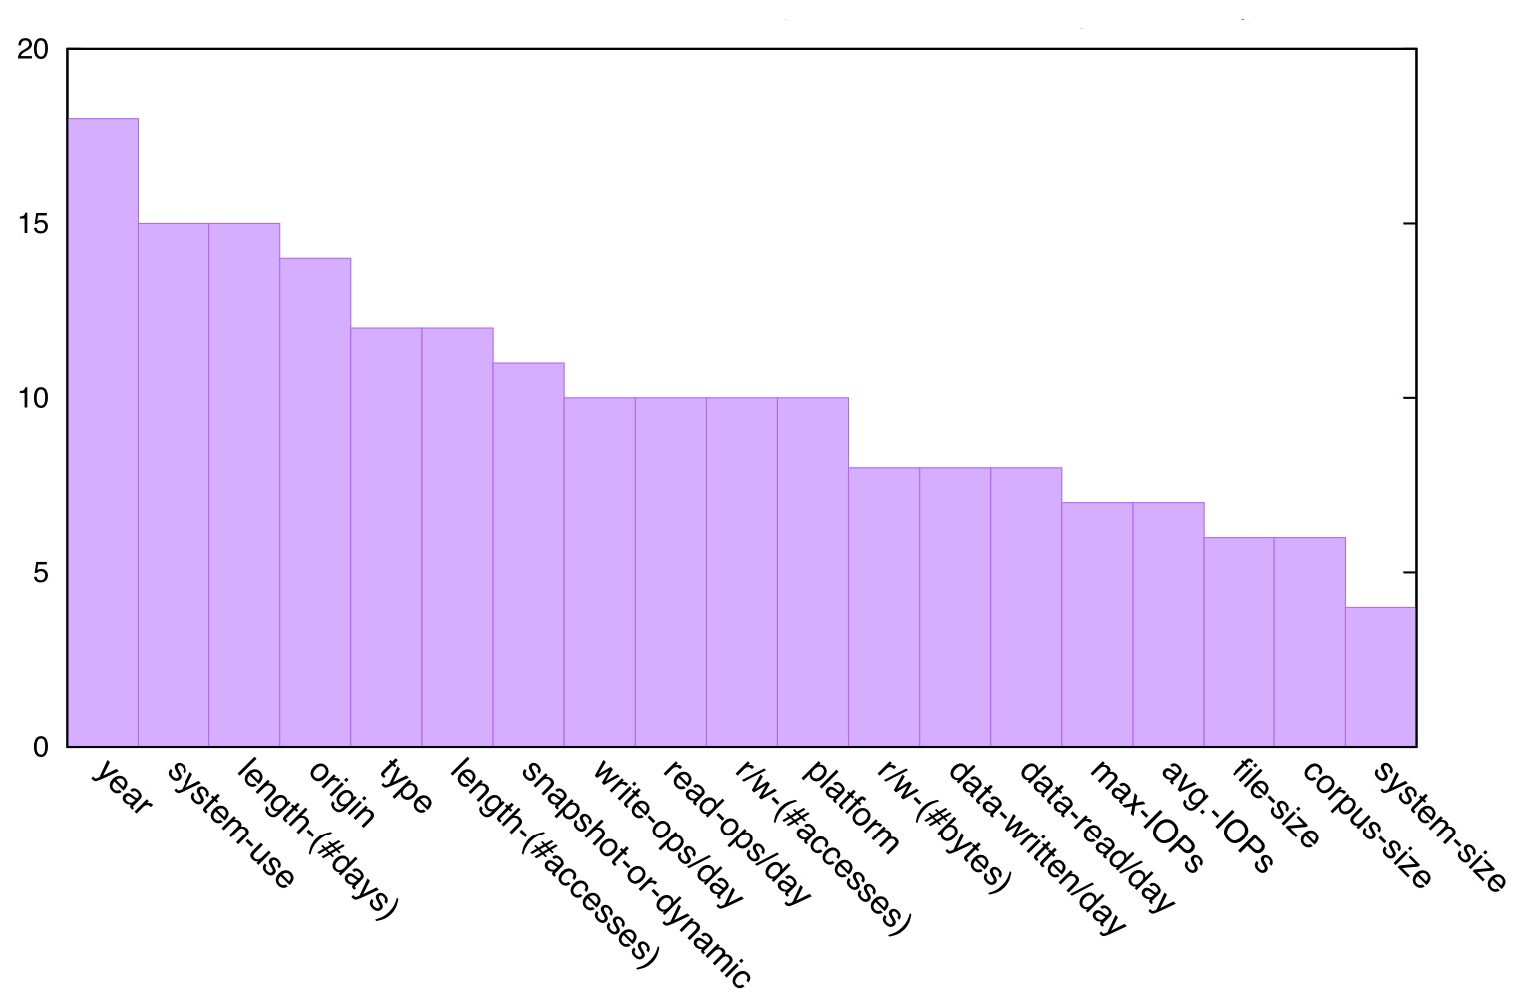
\includegraphics[width=.7\linewidth]{feature_hist.eps}
%\caption{Histogram of popular features collected from 29 workloads}
%\label{fig:features}
%\end{figure}

\begin{table}[h]
\centering
\caption{Common Workload Features}
\label{tab:workloads}
%\scriptsize
\small
\begin{tabular}{lcrrr}
\toprule
\small
Type & Year & Avg.File & \#Reads & \#Writes\\ %& R/W Ratio &
&& Size (MB) &per day&per day\\ %& R/W Ratio &
%Max. IOPS\\
\midrule
User~\cite{dayal} & 1981 & .012 & -- & -- \\%&-- & -- \\
User~\cite{roselli} & 1991 & -- & 207000 & 57000 \\%& 3.61 & --  \\
User~\cite{dayal} & 1993 & .022 & -- & -- \\%&-- & -- \\
User~\cite{dayal} & 1997 & .027 & -- & -- \\%&-- & -- \\
User~\cite{roselli} & 2000 & -- & 303000 & 71000 \\%& 4.27 & --  \\
User~\cite{ellard} & 2001 & -- & 350000 & 438000 \\%& 3.25 & 4719.4 \\
User~\cite{ellard} & 2001 & -- & 19290000 & 5930000 \\%& .8 & 741.67\\
User~\cite{dayal} & 2005 & .327 & -- & -- \\%& -- & -- \\
User~\cite{narayanan2008write} & 2007 & -- & 14847 & 144447 \\%& .0989 & 3925\\ 
User~\cite{dayal} & 2008 & .531 & -- & -- \\%& -- & -- \\
User~\cite{dayal} & 2008 & .37 & -- & -- \\%& -- & --  \\
User~\cite{fiu-dedup} & 2010 & -- & 34593.52 & 814773.19 \\%& 24 & 11897 \\
Enterprise~\cite{roselli} & 2000 & -- & 1270000 & 231000 \\%& 4.49 & -- \\
Enterprise~\cite{roselli} & 2000 & -- & 2320000 & 150000 \\%& 15.4 & -- \\
Enterprise~\cite{dayal} & 2008 & 19.3 & -- & -- \\%& -- & -- \\
HPC~\cite{LLNL03} & 2003 & 3 & -- & -- \\%& -- & --  \\
HPC~\cite{ian-tos} & 2007 & 1 & -- & -- \\%& -- & --  \\
HPC~\cite{dayal} & 2008 & 10.3 & -- & --\\% & -- & --  \\
HPC~\cite{dayal} & 2008 & 15.6 & -- & -- \\%& -- & --  \\
HPC~\cite{dayal} & 2008 & 9.6 & -- & -- \\%& -- & --  \\
Archive~\cite{dayal} & 2008 & 29.0 & -- & -- \\%& -- & --  \\
Archive~\cite{dayal} & 2008 & 21.7 & -- & -- \\%& -- & --  \\
Archive~\cite{dayal} & 2008 & 10.4 & -- & -- \\%& -- & --  \\
Archive~\cite{dayal} & 2008 & 5.2 & -- & -- \\%& -- & -- \\
Archive & 2010 & -- & 1326137 & 595661 \\%& -- & -- \\
\bottomrule
\end{tabular}
\normalsize
\end{table}
To automatically tune storage systems based on projected workload, a clear first
step is identifying the metrics that define the functional relationship between
a workload and the storage infrastructure that serves it.  
%
%
%In addition to a machine-learning based feature selection, we can use domain
%information to better understand what features are most critical for workload
%classification. 

%\begin{wrapfigure}{l}{.5\linewidth}
\begin{figure}
\centering
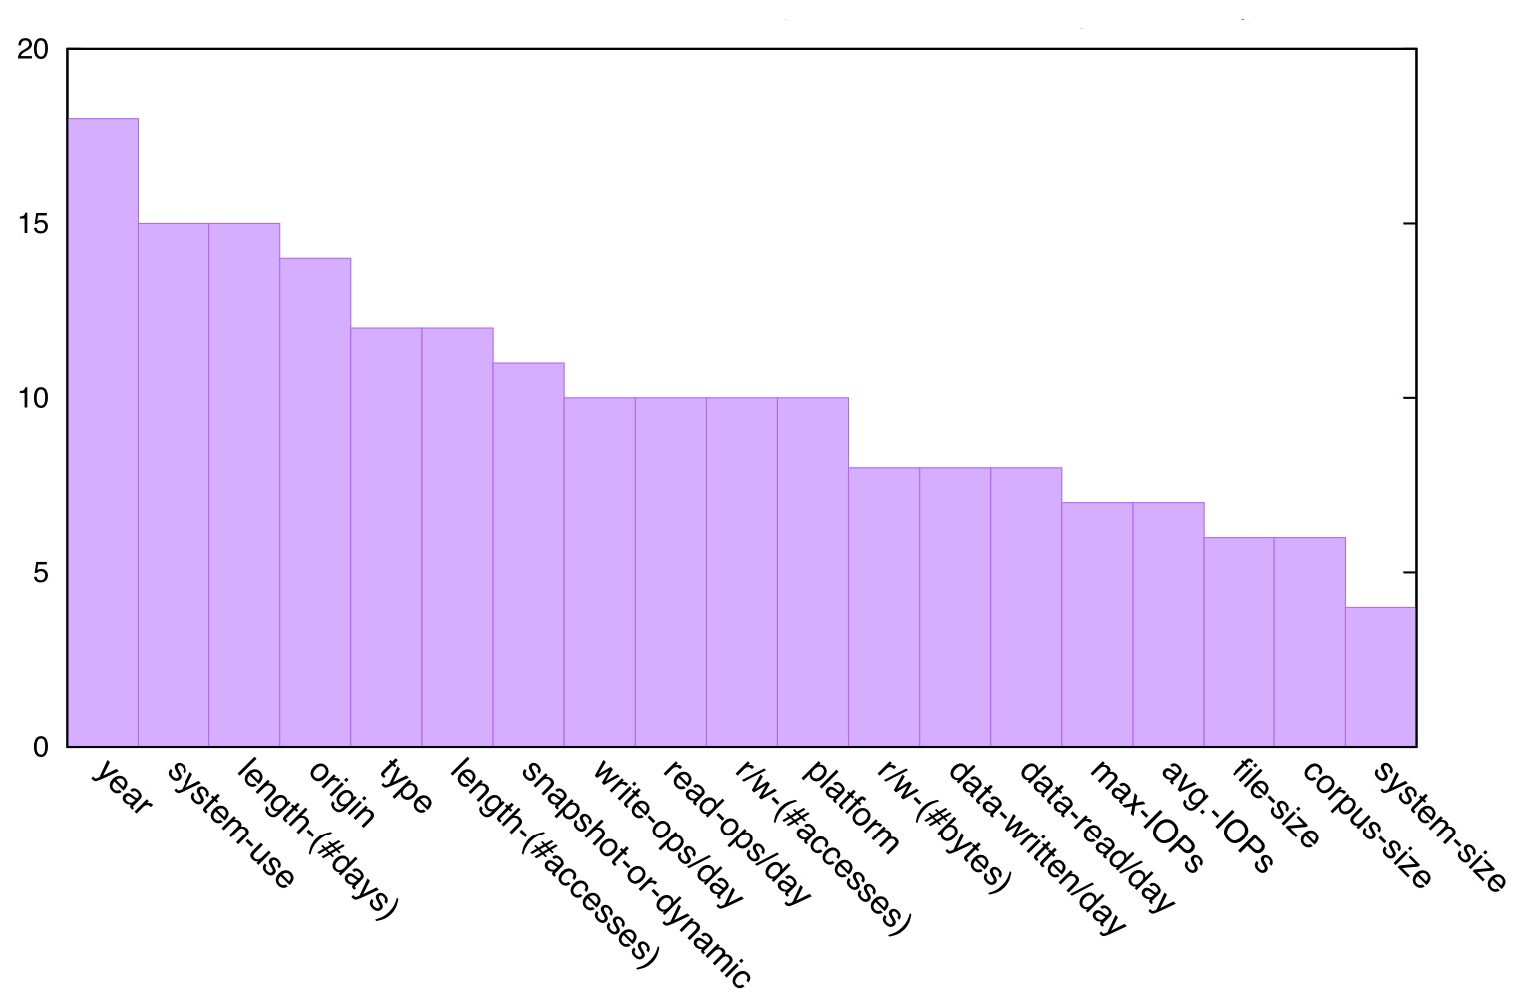
\includegraphics[width=.7\linewidth]{feature_hist.eps}
\caption{Popular features collected from 29 workloads}
\label{fig:features}
\end{figure}
%\end{wrapfigure}
One approach is to consider what workload metrics are most commonly reported in
the research community when proposing novel algorithms and architectures.
We have performed a preliminary meta-analysis
of prior workload studies~\cite{wildani2015case}. Figure~\ref{fig:features} is an incidence histogram of the most
prevalent features from 29 traces that reported metrics.  18 features were reported in multiple workloads, and 5 features were
reported in more than 50 percent of the workloads studied. This sparse reporting of features across previously published datasets is an issue that we will address in this proposal.

Table~\ref{tab:workloads} lists relevant details of previously published
workloads from our analysis. Based on the feature distribution, we see that the literature
appears biased towards metrics such as year and origin that are easy to collect (are these metrics really? You wouldn't put them in a model, right?).
Statistics such as daily reads and writes are also prominent, indicating that
they may be useful for characterization. However,
of the trace analyses we studied, the vast majority of features reported were
only reported for one trace in our sample, indicating that there is a need for a
common set of metrics for describing workload statistics.

\begin{figure}
\centering
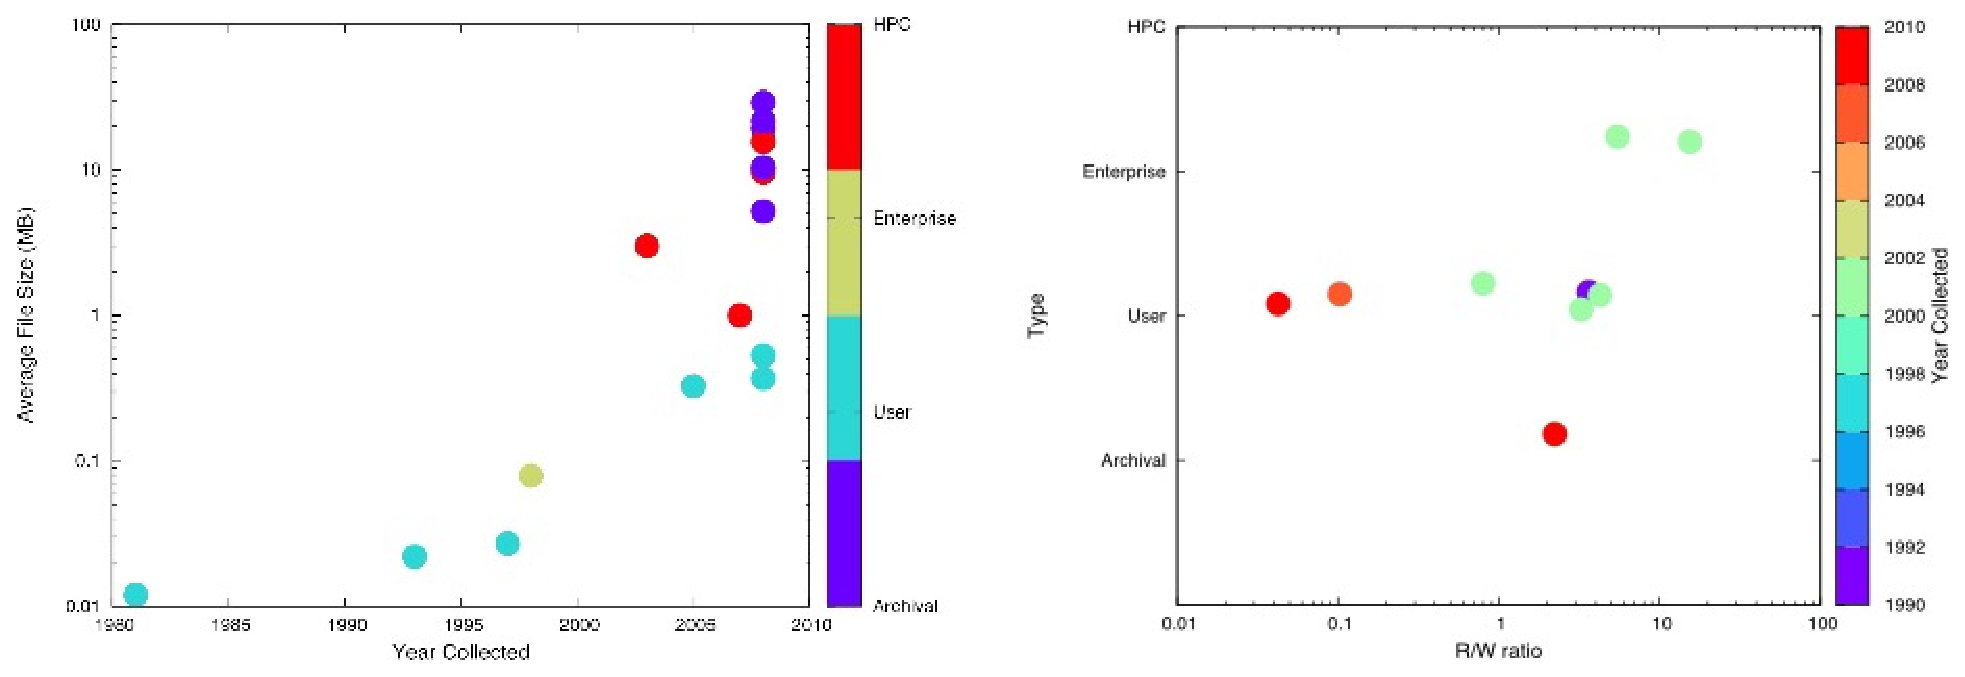
\includegraphics[width=.95\linewidth]{hack.eps}
\caption{``Archival'' traces from the same year have a wide variation in average
file size, while ``User space'' traces vary widely in read/write ratio over time (jitter
added to $y$-axis)}
\label{fig:hack}
\end{figure}

%Figures~\ref{fig:file_size} and~\ref{fig:rw} 
Figure~\ref{fig:hack} shows the discrepancy between the
descriptors used for storage workloads and the characteristics of the workloads
themselves.  The meaning of terms changes both over time and across different
instantiations.  For example, several ``archival'' datasets collected in the
same year (left)%(Figure~\ref{fig:file_size})
show vastly different average file sizes.
%This in turn affects the design guidelines for building and validating an
%archival storage system~\cite{TKSOMEONE}.  
Similarly, designing a workload in
user space that relies on the balanced read/write ratio of older workloads is a
mistake in modern systems 
%(Figure~\ref{fig:rw}),
 (right),
but the terminology describing
the workload remains unchanged.

While the definitions of trace types has changed over
time, the variation in ``archival'' or ``user'' workload characteristics between
traces collected in the same year is a strong indication of the need to create a
more portable and permanent descriptive language to classify workloads.
Additionally, the diversity of features reported in the trace studies that we
examined indicates that trace classification will be both high dimensional and
sparse.  
We propose to extend this preliminary work by adding more studies and tracking what
features of a published trace followup studies rely on when citing the work.
% TODO MAYBE: Add figure for this?
The concept is similar to web ranking~\cite{pagerank}, where repeated references
to a particular concept indicate that that concept is a good ``keyword'' or
descriptor for a document, which in this case is a proxy for the workload the
document describes.

There are a number of reasons why it is difficult to compare and categorize
workloads based on aggregate statistics.  Captured workload data are often based
on the requirements of the local administrator, and thus it is highly variable
between studies and the presence of particular features is not necessarily
correlated with feature importance.  Another tactic we propose to derive metrics
is to leverage the expertise and institutional knowledge of our industry colleagues to create a base OF SOMETHING HERE THAT NEEDS TO BE EXPANDED UPON...

% TODO TALK ABOUT PLAN B: MACHINE LEARNING TO GATHER FEATURES BASED ON GPFS
% TRACES 

\subsubsection*{Data Collection }
% Where is data going to come from?

Establishing a comprehensive storage taxonomy will rely on good data
collection.  Most datasets used to evaluate computer systems are sensitive and
not available to researchers.  However, features of these datasets such as UNFINISHED THOUGHT HERE?


There are two components to the data-gathering phase of our characterization
work: a meta-analysis of published workloads and a statistical analysis of raw
workload data. 

There are a number of reasons why it is difficult to compare and categorize
workloads based on aggregate statistics.  Captured workload data are often based
on the requirements of the local administrator, and thus it is highly variable
between studies and the presence of particular features is not necessarily
correlated with feature importance.  Thus, we also intend to gather a set of
representative workload traces from former and new collaborators to validate the
conclusions of the meta-analysis and help design a robust predictive workload
model.
We will begin by doing a further meta-analysis to track what features have
historically been most relevant to storage systems that were tested with dynamic
workloads.

Beyond this, we plan to use traces from the Storage Networking
Industry Association's Input/Output
Traces, Tools, and Analysis Technical Working Group (SNIA) trace
repository~\footnote{\texttt{http://iotta.snia.org/}} as well as traces
collected on local university servers, traces of medical record databases, and
traces from our collaborators at IBM ARC, Lawrence Livermore National Labs
(LLNL), and Intel Research.
% FIXME make sure you have support letters.



%%%%%%%%%%%%%%%%%%%%%%%%%%%%%%%%%%%%%%%%%%%%%%%%%%%%%%%%%%%%%%%%%%%%%%%%%%%%%%%%%%%%%%%%%%%%%%%%%%%%%%%%%%%%%%%%%%%%%%%%%%%%%%%%%%%%%%%%%%
%\subsection{Preliminary Results}
% FIXME : REMOVED EXPLICIT PRELIMINARY RESULTS SECTION FOR THE SAKE OF THE
% NARRATIVE.
% is it worth separating out classification by feature vs. classification by average stats at this point?

% Commented out for space: we've already got motivation above, so giving this a try.

% Can we find a case where one classification avg closely matches but 
% but the details differ wildly? e.g.''The averages were the same, but the bursts
% and steady state were hugely different? IFA

% Hmm: I don't know. I don't have one up my sleeve atm.  I agree it's an
% interesting question.  Let's hold that thought -- Avani
%\begin{figure}
%\centering
%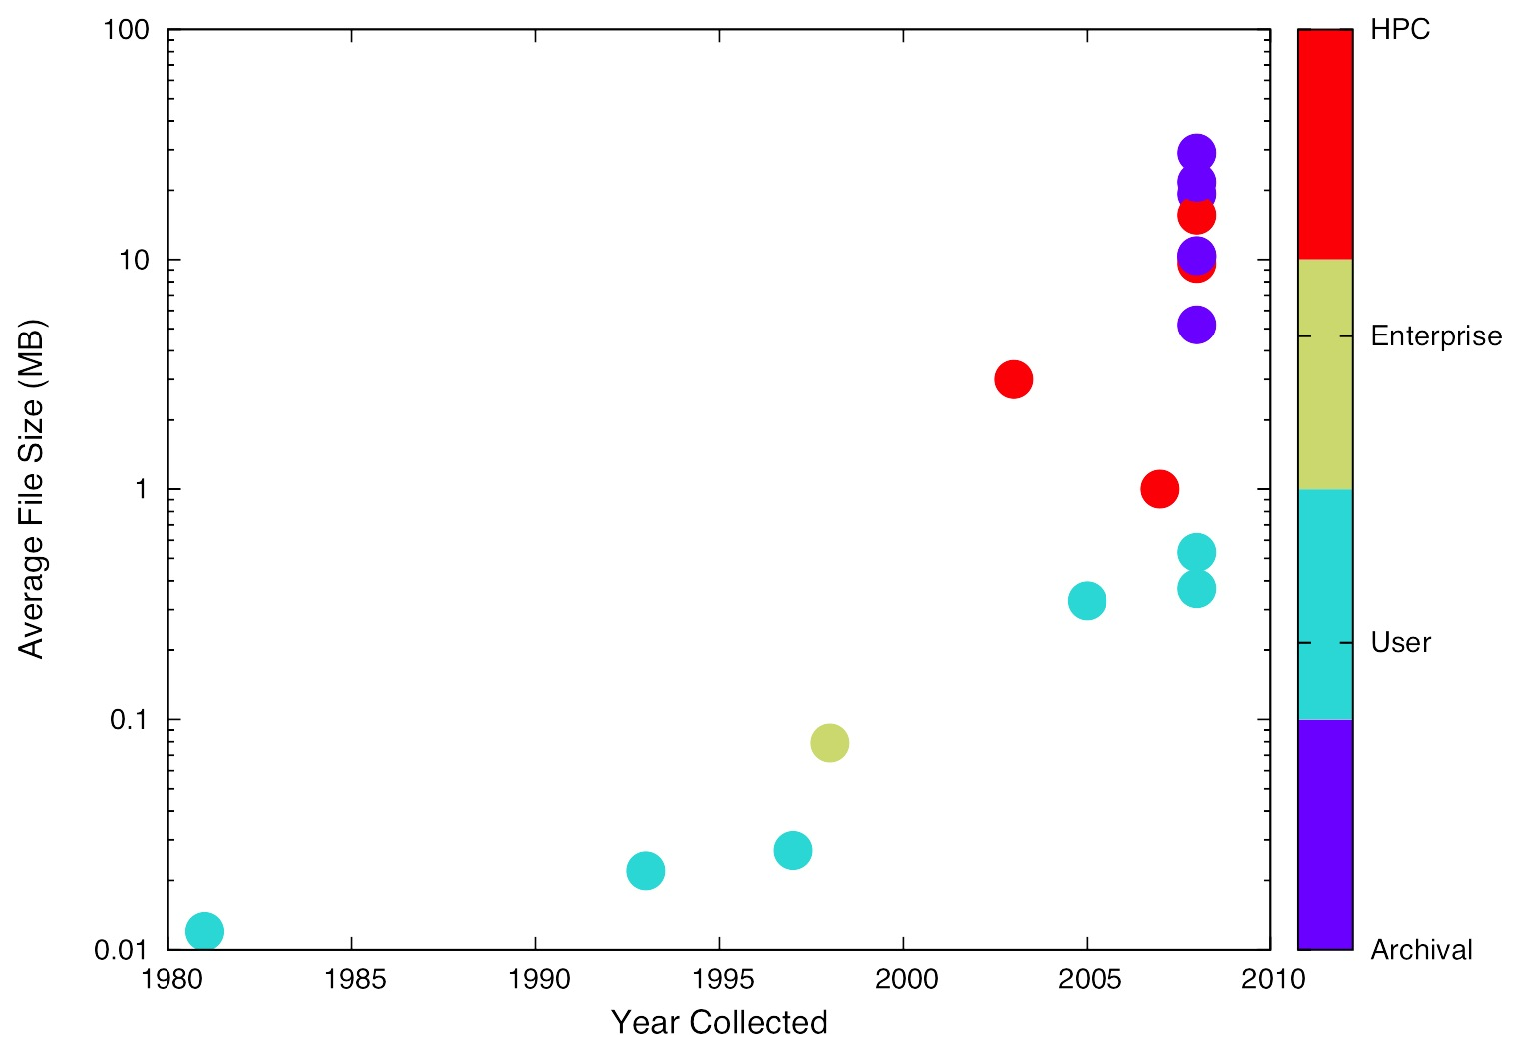
\includegraphics[width=.6\linewidth]{year_vs_avg_file_size.eps}
%\caption{``Archival'' traces from the same year have a wide variation in average
%file size.}
%\label{fig:file_size}
%\end{figure}
%\begin{figure}
%\centering
%\includegraphics[angle=270,width=.6\linewidth]{rw_ratio.eps}
%\caption{``User space'' traces vary widely in read/write ratio over time (jitter
%added to $y$-axis)}
%\label{fig:rw}
%%
%%\caption{Trace features vary both over time and across types.}
%%\label{fig:variations}
%\end{figure}

\subsection{Identifying \MWs}

Given a set of metrics that are known to be interesting to the community and
relevant to the tuning of existing systems, we want to make them useful to the
community.  Multi-dimensional optimization is an intrinsically hard problem, and
moreover the higher-level metrics found by the proposed ML model may not be directly interpretable by an administrator who lacks the time to re-calculate
higher-level metrics on their trace.  Thus, we seek to understand what values
tend to correlate within the metrics we've defined.  We term a set of these
correlated values as a \mW.

%\subsubsection{Going }
 


\subsection{Research Goals}
Having a rigorous, extensible, easily communicable workload characterization
will provide several benefits to the systems community. The characterization
will provide a metric for communicating precise requirements, helping
designers architect systems that are well adapted for the expected workload.
Additionally, dynamic categorization of workloads will allow storage providers
to develop better SLAs that tie performance expectations to storage
characteristics. 
The goal of this quantitative characterization is to develop a method to
identify the features in a trace that best indicate how the corresponding
workload will run on a storage system in the future (We refer to this as the \systemfit).
Feature sets extracted by these methods will be used to make synthetic traces
that will be tested for \systemfit on a storage workload simulator.
%
%Finally, we propose that a quantitative characterization is
%the first step towards more realistic workload simulation and modeling
%IFA-Maybe move this to motivation/background and turn it into prose?
% it actually might be nice as part of the abstract?
% Avani: I like how the paragraph wraps up the discussion and reminds people
% about the motivation.  I feel like if we moved it up the intro would be too
% repetitive
%What can a good workload characterization do?
%\begin{itemize}
%\item Prevent confusion in requirements passing
%\item Help us design systems that adapt to changing workload characteristics
%(tie in quick re-tooling for focus shifts?)
%\item Also help us design systems more specifically to a single workload type
%with rigor.
%\item Design more accurate SLAs for different feature-defined workload types
%\item Allow for more realistic modeling of future workload behavior
%\item Make generated workloads more plausible
%\end{itemize}%}}}

\section{Proposed Research: Automatic workload detection and classification}%{{{

\begin{quote}
Systems programmers are the high priests of a low cult.
-- Bob Barton
\end{quote}

%FIXME Second, within and across the various \textit{types} of workloads, we explore
%the possibilities for common metrics and terminology.  While current
%qualitative labels are convenient for discussion, we extend these types
%through statistical analysis and machine learning

% If you have a single workload, use HMMs to find features.

Once we derive a set of metrics, we need to calculate metrics on traces and
workloads of interest to determine what \mw they most resemble.  We define 
a \textit{workload} as the I/O load produced by a distinct usage of the system.  
However, as storage systems increase in size, multiple workloads sharing the
same space has become commonplace.  
60\% of traces in a recent study included workloads that were strided and
interleaved~\cite{seo_char}.  

% If you have multiple workloads, use ICA to separate.
 A multi-user, multi-application workload is similar to a
noisy party: there are many different ``conversations'' happening in the room,
but we are recording them with a single microphone and we'd like to know who
said what.  Separating out signals by visually examining trace logs is very
difficult, as I/O contention and system activity results in the separate
workloads being mixed even more thoroughly than our cocktail-party example.

Blind source separation techniques like independent components
analysis (ICA) isolate individual non-Gaussian
signals within a shared data pipeline by selecting a set of candidate signals
and then minimizing the mutual information across said signals.     
We believe that ICA could be used to separate workloads as a precursor to
identification.
% TODO Add math, that's why I'm in this godforsaken tex format anyways... :-D  

Our preliminary results (Figure~\ref{fig:ica}) show that ICA
can successfully disentangle workloads in a lab setting.  For both of these
figures, the source traces were converted to signals by whitening and were mixed using
a Gaussian mixing matrix of full rank.
%FIXME Why did you use a GMM if above you say ICA isolates non-Gaussian signals. Is one of these a typo?
The mixing matrix simulates I/O
contention and scheduling issues between the workloads.  
ICA was then used to disentangle the
traces, and mean squared error was calculated to validate the returned traces.  
To validate, we calculate mean squared error (mse) between the recovered signals and
the true source signals.  We found that ICA returned an mse of about 1.30.  To
put this in context, we also calculated the mse for signals returned from
Principal Components Analysis (PCA).  We see, as expected, the mse is
significantly higher for PCA because PCA has an assumption of independence
between signals that ICA does not. 
%FIXME in the real world, do we expect dependence between the signals? In a set with a bazillion users, probably not, but in a smaller one, people/groups/computers often work in teams. How much will that mess with sorting out signals?

\begin{figure}
  \centering
  \includegraphics[width=.99\linewidth]{ica-5pids.eps}
  \caption{5 real application traces~\cite{fiu} were converted to signals and mixed with a
  Gaussian mixture model.  We see both by visual examination and the mean
  squared error (mse: lower is better) that the component signals returned by ICA closely resemble ground truth (note: sign is arbitrary).  The signals
  returned by principal components analysis (PCA), a popular feature extraction
  method, are much less accurate.  Also, while mse was lowest for a long
  trace, even the first ten minutes of I/Os lead to relatively low mse for ICA.}
  \label{fig:ica}
\end{figure}

Separating out workloads and identifying their critical metrics may make it
easier to develop I/O-aware scheduling in domains like super-computing where the
performance variation caused by I/O
resource contention is particularly unwelcome~\cite{liufast14}.

We propose to applying ICA to real systems that lack a
ground truth. 
In particular, ICA takes the number of source signals as a
parameter, and we will be investigating techniques to estimate this number from
an arbitrary mixed workload trace, beginning with the technique proposed in
~\cite{Sparse component analysis and blind source separation of underdetermined
mixtures
}. % There are also alternative mixing models that 

\subsubsection*{Determining workloads from snapshots }
% If you have no block I/O, use snapshots.

Accessing block or filesystem-level I/O traces is occasionally difficult.
Tracing is often not enabled by default, and retaining traces for larger storage
systems creates a non-negligible I/O footprint that will bias an automatically
generative model of the workload. 

Metadata snapshots are a common method for gaining insight into filesystems due
to their small size and relative ease of acquisition. Since they are static,
most researchers have used them for relatively simple analyses such as file size
distributions and age of files. These snapshots are also typically much smaller,
and consequently easier to collect and store without undue system impact, than
dynamic traces.  For HPC systems and other applications where dynamic trace
collection is infeasible, we plan develop a novel two-step method to use
metadata snapshots for characteriztion: \textit{separating} interleaved
workloads by \textit{clustering features} in snapshots and then
\textit{classifying} the workloads based on a \textit{convolutional neural
network model}.

With the basic POSIX-like metadata produced from a \texttt{stat} (or similar
command) of the files in the system, one can glean a variety of useful
statistics of interest to researchers and administrators, such as file size
distributions and namespace layout. With multiple snapshots taken over time, it
is even possible to see how file systems evolve~\cite{agrawal:fast07} or to
calculate the inter-reference intervals between files~\cite{gibson:cmg98}.
Since these metadata snapshots are typically much smaller than dynamic traces,
static metadata is relatively easy to collect quickly and store
semi-permanently. This size advantage, along with the lower performance overhead
for collecting static snapshots, makes them relatively easy to obtain for
analysis.

Unlike dynamic traces, snapshots do not
suffer from arbitrary gaps or incorrectly ordered accesses due to tracing bandwidth limitations.  That said, snapshots are not taken atomically, and so all temporal
correlations are assumed to be within a margin of error proportional to the size
of the file system. 
% FIXME Replace with something about how clusters would help us realize
% high-importance features / l2 hidden features and also how clusterings may
% correspond to actionable workload characteristics. 

%As an example, consider trying to identify the access locality within a file
%system. %maybe cite groupingy stuff 
%If files track their last modification time with
%reasonable accuracy, we can take a simple two step process to start learning
%about their modification locality. First, we group files by similar modification
%times, using a density based technique such as DBSCAN~\cite{ester:kdd1996}. We
%can then analyze each of these clusters along a variety of dimensions. It can be
%as simple as comparing the number of unique user IDs within each cluster to see
%if UID is a good predictor of modification locality, to more in depth techniques
%such as agglomerative clustering to examine the namespace locality within files
%modified at a similar time.
\subsection{Preliminary Results: }
Metadata snapshots present us with a highly non-linear, multidimensional
data set.  To meaningfully compare snapshots and discuss correlations within
them, we borrow the concept of a \textit{view}~\cite{mascotssnapshot}.  A view is simply a
projection of the snapshot space onto three dimensions.  Views allow us to
visually isolate different aspects of user locality, such as when users modify
files they created, and help define what clustering
algorithms are likely to perform well on each snapshot.
%\begin{figure}
%\centering
%\subfigure[\texttt{archive}]{
%\includegraphics[angle=270,width=.42\linewidth]{actual-n10-uid-create-mod.eps}}
%\subfigure[\texttt{gnfs}]{
%\includegraphics[angle=270,width=.42\linewidth]{actual-n10-uid-create-mod_gnfs.eps}}
%\subfigure[\texttt{lnfs}]{\centering
%\includegraphics[angle=270,width=.42\linewidth]{actual-n10-uid-create-mod_lnfs.eps}}
%\caption{Create time vs Modification Time views of LANL snapshots with the top 10
%UIDs identified by color.  The concentrations of accesses by the same UID
%represent the type of patterns unsupervised learning should find.}
%\label{fig:n10-u-c-m}
%\end{figure}
%Metadata snapshots present us with a highly non-linear, multidimensional
%data set.  To meaningfully compare snapshots and discuss correlations within
%them, we introduce the concept of a \textit{view}.  A view is simply a
%projection of the snapshot space onto three dimensions.  Views allow us to
%visually isolate different aspects of user locality, such as when users modify
%files they created, and help define what clustering
%algorithms are likely to perform well on each snapshot.

\begin{table}%\footnotesize
\centering
\small
\caption{LANL Snapshot Statistics}
\begin{tabular}{llcc}
\toprule
&Type&\# Records&\# Machines\\
\midrule
\texttt{archive}&Archive&112020366&13\\ 
\texttt{gnfs}&Global NFS&6437081&13\\
\texttt{lnfs}&Local NFS&306340&2\\
\bottomrule
\end{tabular}
\label{tab:datasets}
\end{table}
\normalsize

We examined a series of views using three anonymized snapshots from Los Alamos
National Laboratory (LANL); Table~\ref{tab:datasets} contains details.    
From these snapshots, we focus on the fields ``create\_time,'' ``modification\_time,''
``UID,'' ``group\_id,'' and ``file\_id'' to explore user locality.
%The other fields, ``block\_size,'' ``size,'' ``path,'' and ``permissions,'' were
%either low information or non-numeric, making them less 
%The snapshots were
%anonymized such that the path field indicated level within the directory hierarchy.
To analyze storage snapshots, we need an unsupervised learning algorithm that can support $n$-dimensional, non-linear heterogeneous data with low inter-cluster separation while ideally encoding hierarchical relationships between both data and labels without overfitting.
Additionally, our algorithm should handle arbitrary numbers of sparse, binary
dimensions to encode Boolean queries about the files in the snapshot
, such as queries over the ``permissions'' and ``path'' fields.  


Agglomerative clustering is a well established, interpretable unsupervised
machine learning algorithm that fulfills all of the requirements for snapshot
analysis as well as providing a natural hierarchy for correlating user locality with path.  We also tested $k$-means and a simple grouping based on a single attribute at a time. 
% TODO: Decide if we also want iClust in this.

To measure cluster validity in the absence of ground truth, we calculate the joint Shannon entropy across a set of features of
interest within each clustering.  In the preliminary work represented in
Figure~\ref{fig:clusterings},  we calculate a mean entropy defined as
$$H_{snapshot}=\frac{\sum_{f\in F}{\sum_{i \in C_f} \[-\frac{N_i}{N}\log_2{\frac{N_i}{N}}\]}}{|F|}$$
where $F$ is the set of snapshot features, $C_f$ is the set of possible values
for the instance, $N_i$ is the number of samples that show value $i$, and $N$ is
the total number of samples.
\begin{figure}
    \centering
    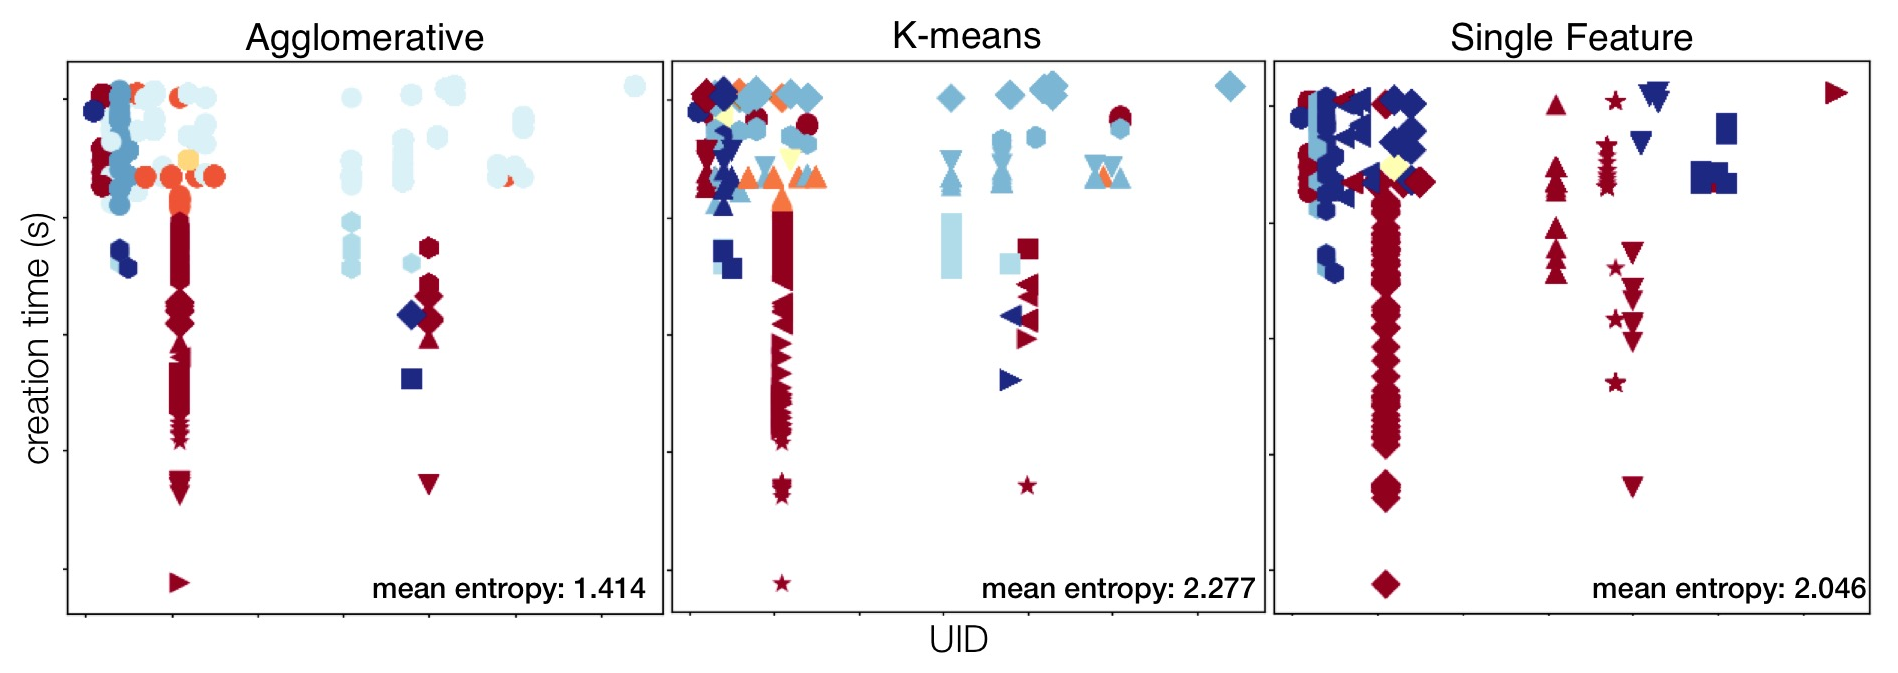
\includegraphics[width=.95\linewidth]{hotstorsnapshot.eps}
    \caption{Sample clusterings and entropies for a single snapshot view.
    Clusters are indicated by shape and modification time is indicated by color.
    Lower entropy numbers indicate better clusterings.}
    \label{fig:clusterings}
\end{figure}
We examined a series of clusterings using HPC and archival snapshots from Los Alamos
National Laboratory (LANL) and a set of workstation snapshots collected at Emory.
Figure~\ref{fig:clusterings} shows a representative LANL snapshot under
different clusterings. As expected, agglomerative clusterings have lower mean
entropy.    

Based on these results,
we
are investigating clustering algorithms such as iClust~\cite{TK} that can
be calculated on-line and support $n$-dimensional, non-linear heterogeneous data and data with low
inter-cluster separation.
\end{itemize}

% *** Put these in the real paper *** 
%\begin{figure}
%% Histogram of files in different directory levels?  
%\end{figure}
%
%\begin{figure}
%% In-directory entropy wrt to GID, UID, size?
%\end{figure}
%
%\begin{figure}
%\centering
%\subfigure[\texttt{archive}]{
%\includegraphics[angle=270,width=.42\linewidth]{actual-n10-uid-gid-mod.eps}}
%\subfigure[\texttt{gnfs}]{
%\includegraphics[angle=270,width=.42\linewidth]{actual-n10-uid-gid-mod_gnfs.eps}}
%\subfigure[\texttt{lnfs}]{
%\includegraphics[angle=270,width=.42\linewidth]{actual-n10-uid-gid-mod_lnfs.eps}}
%\caption{Group ID vs Modification Time views of LANL snapshots with the top 10
%UIDs identified by color}
%\label{fig:n10-u-g-m}
%\end{figure}
%
%Figure~\ref{fig:n10-u-c-m} shows the ten most popular UIDs (re-labeled as 1-10), represented by color, graphed
%against file creation and modification times within our three snapshots.
%Remaining UIDs were placed into a separate group, ``Other'', represented by
%UID 11.  
%Since we are at an early stage in our work, we have focused on views of our data
%sets that provide the most evidence for interesting user locality behaviors.  Each graph represents an entire snapshot, though for clarity we
%subsample by only plotting every hundredth snapshot entry.  The shapes and
%locations of the apparent clusters are driving our search for a high validity
%clustering method that is generalizable to other snapshots with minimal
%parameter selection.  As such, at this step we are focusing on high level
%patterns that are representative of the trace.


%We
%restrict our preliminary analysis to high activity UIDs to obtain a sense of
%how much noise our clustering algorithms will need to tolerate.  In the
%\texttt{archive} snapshot, we see distinct clusters of file creation by the same
%user -- for example the vertical line of blue accesses at approximately
%$1.2\times10^9$ seconds.  We also see a range of users creating files late in the time
%covered by the snapshot.  The \texttt{gnfs} case shows a few outlying creates that happen
%a long time after most do.  We also see a very
%different modification pattern compared to the archival case; instead
%of many modifications by a user mapping to the same create time, we see the
%opposite, horizontal bands of user creation activity across a single
%modification time.  Moreover, these bands overlap.  This indicates that any
%clustering that accurately classifies usage requires more than three
%dimensions to separate distinct user groups.  In terms of real usage patterns,
%the vertical clusters of the \texttt{archive} case could be a log file, whereas
%the horizontal clusters of \texttt{gnfs} could correspond to batch processes on
%the shared filesystem.  

%Finally, the \texttt{lnfs} case shows a local system with the high activity
%$users doing almost all of their file modifications within a very small window of
%time.  This indicates a very active system, where files are touched frequently, in contrast to the archival system where there is a large spread of
%modification times between users.  Other views we have taken of these
%snapshots, including looking at UID and modification time plotted against
%File\_ID or Group\_ID (Fig.~\ref{fig:n10-u-g-m}), follow very similar patterns.
%In the Group\_ID views, for instance, we see that popular users are generally only
%modifying files that belong to one or two groups, and, particularly in the
%\texttt{lnfs} case, most of these modifications are within a small span of time.


%% Discuss this in real paper!
%Additionally, our clustering should handle arbitrary numbers of sparse, binary
%dimensions to encode ``yes/no'' questions about the files in the snapshot
%5derived from the permissions and path fields.  

\subsection*{Research Goals: }
%Clustering a single snapshot is a novel approach that is
%useful given the size and performance requirements of modern systems. 
%We believe that our clustering will be able to hint at working
%sets based on modifications grouped by labels such as user or path.  These
%working sets could then reveal hidden characteristics of a workload, such as
%project interrelationships, from a single snapshot.    
Given enough data, our ultimate goal is to reliably classify snapshots
by the type of workload they represent. Once we are satisfied with the clustering metric, we will build a neural network to determine what \mws the various clusters most represent. 
Neural networks are %FIXME
%FANTASTIC.  THEY SOLVE ALL THE PROBLEMS AND DEEP LEARNING BUZZWORD.  Also, I can point to my brain stuff here which is otherwise totally unrelated. hahahaha. awesome.  But, perhaps, at a minimum... make this a full sentence.

\begin{figure}
    \centering
    \includegraphics[width=.7\linewidth]{nn-example.eps}
    \caption{This example network classifies audio samples.  We converted the high dimensional source data to a spectrogram and built a CNN.  Note that the intermediate, hidden nodes in the graph, represented by the lower row of images, correspond to complex features instead of single notes.  When played, these form recognizable motifs, leading us to believe the same concept could work for storage workload snapshots.}
    \label{fig:nn}
\end{figure}

Moving further, we would like to combine the clusterings from a single-snapshot
analysis with the methodologies in place, such as learning inter-reference
intervals, to learn trends between snapshots.
%FIXME You might comment about figuring out how many snapshots/what intervals you'd need for this to be feasible. 
For instance, we could compare a
%FIXME I like concrete plans better than 'could'
series of clusterings to refine the clustering parameters.  Finally, we are
interested in studying the effect of changes in snapshots on the clustering to
obtain a rigorous validity metric.
%}}}ii
% We have another short paper to stick in here!
\section{AutoTune: Raising the Storage Bar With \Mws}%{{{


In the third phase of this project, we will build a set of parameterized configuration
recommendations for \mws and develop an infrastructure aware distance metric
that will answer the question ``given the workloads I have, what tuning
parameters should I start with?''

There is a cold-start problem here: how do we know the properties of a new
workload before we've built a system to run it?  

To solve this problem, we remember that workloads correspond to a real set of
actions that users or applications need to perform to accomplish some reward
function.  A generic way of expressing this reward is a set of Service Level
Agreements (SLAs), which are objectives (\eg ``serve 80\% of requests out of
cache'') paired with costs for not meeting the objectives.  We propose to
jump-start model selection by selecting the most important objectives, weighted
by the cost, as metrics to compare against our \mws tree.



we will take our functional basis vectors,
our \mWs, along with the workloads we mine, %FIXME and make some full sentences that start with capitalized words and end in periods.


The goal of the workload characterization proposed in this project is to lay
the groundwork for an adaptive storage framework that can suggest a 
storage system design optimized for the relevant features of a workload, including elements such as storage media, network
connections, or data migration policies.  We will simplify the multi-dimensional
optimization framework by developing a notion of \systemfit between specific
high-information features of a workload and the system characteristics that
impact those features.  %Note that features that best characterize a wo

If our workload features are extractable and high information, as a stretch
goal we propose to derive a probabilistic model to track feature stability of workloads and understand shifts over time. We will use a
probabilistic graphical model that updates itself by periodically sampling the
workload and using the  as the reward function for a
reinforcement learning-based update.  Potential models include dynamic Bayesian
networks with feedback~\cite{poupart2006analytic} and factor
graphs~\cite{lecunfactor}.  

%For example, a
%workload may be characterized primarily by having a 99\% likelihood of write
%size being between 4KB and 8KB and a $< 2$\% likelihood of data overwrite or
%5delete.  A system that made writes efficient at the expense of deletes, such as
%LFS~\cite{lfs}, would have a high \systemfit for this hypothetical workload.


\section{Prior Work by the PI}
%FIXME
%%The PI's current and prior research spans networked systems, data analysis and information security. 
Characterizing workloads aligns closely with the PI's research vision of \textbf{quantifying storage provisioning}:
%\textbf{\emph{automatically finding the best ways to disseminate information to multiple parties in diverse system environments}}.

This CAREER proposal outlines a roadmap towards unsolved research challenges of understanding low-level storage patterns/interactions and developing adaptive storage system frameworks.  The PI has published preliminary results for feature isolation and workload characterization~\cite{wildani2015case,TK_MASCOTSSNAP,TK_HOTSTORSNAP} as well as initiated and chaired the Workshop on System Analytics and Characterization (SAC), which was co-located with SIGMETRICS in 2016, to reach out to the systems community and understand current unsolved issues in workload characterization~\footnote{https://sites.google.com/site/sacconference2016/index}.     

Finding patterns in storage systems has been central to the PI's research program~\cite{avani-systor,TK_tos}, ranging from exploiting patterns for power management~\cite{avanipdsw}, grouping hashed blocks to reduce the disk bottleneck in in-line deduplication~\cite{hands}, to finding daily usage patterns in industry workloads to reduce the monetary impact of disk rebuild~\cite{perses}.   
%smart data replication within caching;
%papers demonstrating preliminary results of \smartcache{}'s performance profiling \cite{saemundsson2014dynamic} and 
%regenerative cache \cite{sigurbjarnarson2014harmonium} have been published, showing feasibility of these approaches.
%The scalability of data replication in large-scale distributed systems has been the backbone in the PI's research,
%ranging from work on distributed caches \cite{sigurbjarnarson2014harmonium,saemundsson2014dynamic,huang2014characterizing,chockler2011design},
%live video streaming \cite{friedman2014molstream,vigfusson2012brief},
%multicast \cite{vigfusson2010dr,huang2010kevlar,huang2010quilt,basin2010sources} to other protocols 
%\cite{vigfusson2010optimizing,vigfusson2009go,girdzijauskas2010magnet,abulibdeh2013leveraging},
%with several highly cited papers on the subject \cite{vigfusson2010dr,girdzijauskas2010magnet}.

%The PI's thesis on data replication was \textbf{nominated for the ACM Doctoral Dissertation Award}.
%
%In addition, the PI has worked on data analysis and machine learning \cite{vigfusson2009adaptively,gudmundsdottir2014extending,rovelli2014pmds,thesis}, including a project of characterizing load imbalance across Facebook's memcache servers \cite{huang2014characterizing}, as well as security
%\cite{rovelli2014pmds,johansen2014fireflies,guerraoui2012decentralized,jonsson2012secure,jonsson2012robust}, including work for which his Ph.D.~student received a Best Student Paper award \cite{jonsson2012bootstrapping}.
In addition, the PI has worked on data analysis and machine learning~\cite{GAUL,TK_Env,TK_?,TK_tos,TK_thesis}, including neural computation techniques that explored feature detection in biological systems~\cite{TK_Tanya}.  

%\begin{itemize}
%\item The PI has advised several students on computer security, including one Ph.D.~student, which has produced several publications 
%He also benefits from 
%Through the previous research, the PI has developed a set of skills in a number of interrelated areas,
%ranging from systems building to mathematical modeling and statistics. 
%He will leverage the skills, and the lessons learned in the past research experiences, to address the challenges
%of the proposed research.



%}}}i

%%%%%%%%%%%%%%%%%%%%%%%%%%%%%%%%%%%%%%%%%%%%%%%%%%%%%%%%%%%%%%%%%%%%%%%%%%%%%%%%%%%%%%%%%%%%%%%%%%%%
\section{Related and Complementary Work}%{{{i
\label{sec:related}

% Workload labels are borked-More details
%IFA-Still got a lingering TODO, would your semantic data placement/power aware 
% work fit there? Anything from Yan Li or Chrissy?
\subsubsection*{Workload Characterization: }

Even from a qualitative standpoint, workload labels are, at best, vague.
Consider the term ``archival''. Venti considered archiving to be more akin to
long-running backups/versioning~\cite{venti}. Adams \etal considered
archives to be long-term historical and scientific data~\cite{ian-tos}, while
the authors of the Pergamum system considered archival data to have the ``write-once,
read-maybe'' semantics typified by financial compliance data~\cite{storerfast2008}.
Similarly, Chen \etal showed that there is wide feature disparity in the space
of user traces~\cite{chen-kmeans}.  ``HPC'' workloads have transitioned from
only performance constraints to both performance and power
constraints~\cite{hpcpower}.  Finally, Wildani \etal showed that workloads
in a multi-use system may be interleaved~\cite{hands}. 

One metric developed in the absence of characterization is ``relative
fitness.''~\cite{mesnier07}.  Relative fitness measures the improvement from
moving a known workload between two infrastructures.  Measuring improvement
allows for insights about suitability for an infrastructure to a given workload
without having to go through a full parameterization, but it ultimately is a
low-information metric that fails entirely if the workload properties are
dynamic or if the systems in question are vastly different.  It also does not
suggest further areas of improvement.

\subsubsection*{Trace Collection: }
Chen~\emph{et al.} pointed out that
the mechanism for trace collection has an outsize impact on the eventual
classification of the trace~\cite{chen-kmeans}.  To take an extreme
example, a database workload that is traced after all of the sequential accesses
have been removed is essentially noise, whereas the same workload traced at a
lower level of the storage stack shows a recognizable access
pattern~\cite{hands}.  As such, the encoding of workload statistics must be
level-aware; traces should only be compared against traces taken at similar
levels unless a quantitative mapping exists between classes at different points
in the storage stack.  


Another feature of quantitative workload analysis is adaptability.  Once we
transition to a more granular, unified model of workload characterization, we
will be able to better detect changes in the usage patterns of workloads as they
inevitably shift over time.  Cherkasova and Gupta~\cite{char_local} characterize the
evolution of two enterprise workloads, and even with such a small sample set see
significant variation over time in the number of unique clients and popularity
of new files.  If we replace a single workload label with a set of features, we
can track shifts in features individually over time and adapt the system to best
fit the workload.  Other previous work has attempted to separate traces by sequentiality and
proportion of interleaved working sets~\cite{seo_char}.  


%for improvement. 

\subsubsection*{Workload Generation: }
Workload generators, such as YCSB~\cite{ycsb}, may fail to model effects that
exist in real
data, but remain critical given the difficulty of collecting rich storage traces~\cite{memcached-sigmetrics,ganger1995generating,kurmas2003synthesizing,tarasov2012extracting}.  
Chen \etal~\cite{chen-kmeans} performed a feature-based analysis of enterprise
storage traces to examine storage traces at multiple layers in the storage
stack as well as to perform feature-based trace analysis.  They claim that
feature selection requires domain knowledge, which we disagree with based on
the work of~\cite{powers}, which showed that features derived from one workload
were generalizable to new systems that lacked domain-specific data.
% We want to point out that there is no reason this problem domain is different
% from domains such as signal processing where blind feature separation is a
% well studied area. 
%I Like it IFA
While they support a multi-variate analysis of workload features, the $k$-means
analysis they perform makes several assumptions about the distribution of
workload features that do not generalize to other datasets. %or work at all,
% the frauds.  Seriously?  They just picked a bunch of centers and saw where
% bubbles fit the best?  That is idiotic.  
This is a fundamental limitation of the $k$-means clustering 
algorithm~\cite{robinson}.
Mesnier~\etal propose a metric of ``relative fitness'' in storage to abstract
away the feedback between storage workloads and system
design~\cite{mesnier05,mesnier07}.  
% Also, this paper is total shit.


%%More papers
%\begin{itemize}
%\item multi-workload studies
%\item vasily's trace replay stuff : this is an application of workload
%characterization that we think is critical but that we don't address in this
%work
%\end{itemize}

\subsubsection*{Trace Analysis: }

A number of recent studies have used dynamic traces of storage systems to
identify working sets~\cite{doraimani2008file,hands}.  Identifying working sets
accurately and reliably can greatly improve both the performance and the
efficiency of storage systems~\cite{bhadkamkar2009borg}.  Additionally,
understanding workload characteristics is essential for optimal storage
management and provisioning~\cite{ian-tos}.

Keeping complete logs of accesses is prohibitive in many systems, however,
because of the computational overhead to collect the logs and the storage
overhead to keep them.  For a modern storage system with hundreds of thousands
of I/Os per second, storing even minimal representations of the I/O without any
metadata is very costly.  For example, an enterprise storage system creates over
16~GB of block-level I/O logs per day~\cite{hands}.
% In hands, we give the IOPS number of about 200,000.  To get the 16GB, we
% assume a byte / access.  This is actually vastly under what it really was, but
% that's an unciteable number.  Maybe rephrase to include calculation if we
% care.

Storing metadata is even harder than storing raw accesses because there
is more overhead both in terms of size and performance.  As a result, metadata
is almost exclusively stored as snapshots -- static read-outs of stored data
elements along with metadata such as \atime, \ctime, and \texttt{path} -- and most
analyses attempt to interpolate dynamic traces from these snapshots.  

% You can learn a lot between snapshots
For example, Gibson and Miller~\cite{gibson:cmg98} calculate inter-reference
intervals from daily snapshots to
obtain long term trends.  While their work contained valuable insights, such as file
usage over time, they require dynamic data and remark that they met resistance
from system administrators when requesting even a
daily trace.  
Similarly, Agrawal \etal~\cite{agrawal:fast07} performed a long-term study of file system metadata using annual
metadata snapshots from thousands of enterprise desktops.  They were able to
watch the changes both of their users and the file system, utilizing a very large dataset.  Our work to identify
trends within snapshots augments this type of work; for example, clusters could
be tracked across multiple snapshots to track how the apparent usage patterns
change over time.

% interpolating snapshots has limits, and we avoid making those assumptions when
% we look at single snapshots?
%      % But there are limits
%Adams called out shortcomings of snapshots


  % What about working with single snapshots?
One area that has been analyzing single snapshots of systems is computer
forensics.  Often, the goal in a forensics environment is to identify particular
files or users that are anomalous compared to the rest of the
snapshot.  Many of the techniques these researchers use apply
to our problem.  For instance, Rowe and Garfinkel~\cite{rowe:icst11} point out that
files that have close proximity in creation or modification times can have
causal relationships, and they also look for co-occurrence of files that are
duplicated in a snapshot.                

\subsubsection*{Dynamic Storage Management: }
There are a multitude of projects that aim to dynamically reconfigure storage
systems in response to particular shifts in usage or resources.  A rigorous
workload characterization will improve the guarantees that these projects can
make by better predicting the future expected workload.  
Zadok \etal{}~detail how automatically reducing storage consumption 
can decrease management overhead and device lifetimes in a multi-user environment
\cite{zadok}.  
The Cake project aims to enforce service level objectives on shared storage
systems through a tiered, dynamically updated scheduling system~\cite{cake}.
Soundararajan~\etal focus on dynamically allocating resources for database
workloads, and show that on-line modeling of these workloads is possible and
that these models improve the performance of virtualized storage
environments~\cite{soundararajan2009dynamic}.  
Many other ``black-box'' storage performance models assume static
workloads~\cite{hippodrome,gulati2011pesto,kelly2004inducing,wang2004storage}.

%They modify a file system to maintain elastic disk quotas by enforcing 
%compression, downsampling or removal policies of certain file types when
%a user's quota is exceeded. 
%The removal policies are akin to our \motif{}s, except without programmability
%or support for precomputation or wider consideration of fungibility, such as 
%network resources.
%

%Nectar is a distributed system
%that manages the storage volumes used for dataset computation within 
%data centers \cite{nectar}. It 
%automatically and transparently removes unneeded intermediate datasets that
%fill up space, and recomputes them from the original dataset and a LINQ program later if needed. 
%%Computation in Nectar involves a series of functional transformations from original datasets, resembling stream processing. 
%Nectar explicitly explores the data-computation trade-off, but
%unlike \smartcache{} it makes fundamental assumptions that restrict the generality of input data, the execution environment and the generality of computational transformations.

%Network storage and archival file systems have
%long been used to store data no longer required to live on primary storage.
%These systems are commonly LAN-based \cite{ori,cimbiosys} but
%personal cloud storage services such as DropBox \cite{dropbox}
%have gained popularity. Most of these systems replicate the content
%on both systems, commonly for backup and robustness purposes,
%and do not automatically offload content to save space on the primary storage.

Several distributed systems balance performance with storage overhead.
SpringFS \cite{xu2014springfs} changes the number of active storage servers
depending to meet elasticity and performance targets, passively migrating
data in the background.
Sierra \cite{sierra} and Rabbit \cite{amur2010robust} seek to reduce power consumption
of their systems by manipulating storage. % XXX%}}}

\section{Success Metrics, Implementation and Evaluation Plan}%{{{

Project success in terms of research impact,
systems building, and broader impacts will be assessed annually. 

\subsubsection*{Metrics: }

%Metrics for metric generation
 % Metrics are going to be judged based on if they're both interpretible and if 
Features are determined to be characteristic of a workload if they are
\emph{high-information}, defined using \emph{Shannon entropy}, for a given workload stream in a mixed-workload environment.  This
means that the metric in question \emph{maximally separates} two workloads that are
known to have different requirements.  We will test this separation using both
generated workloads w


%  We
%will perform an independent component analysis to verify that the features produced
%are the best fit for the workloads sampled.

% FIXME Metrics for separatoin


% FIXME Metrics for workload characterization/fit
%The primary metric for evaluating how well a system is provisioned for a
%feature-defined workload will be \systemfit. 
%Empirical evaluation of systems with high \systemfit will compare these systems
%against systems using traditional workload prediction using metrics including
%\emph{system load}, \emph{power consumption}, and \emph{I/O latency}.

The primary metric for learning and performance profiling is the
\emph{accuracy} of the estimated distribution to an optimal curve.
Once
we separate workloads, we can test that the metrics we selected are the optimal
metrics to divide our workload space.
Empirical evaluation of systems tuned with seperated workloads will compare
these against tuned interleaved system% using metrics including
%\emph{system load}, \emph{power consumption}, and \emph{I/O latency}.
%  We
%will perform an independent component analysis to verify that the features
%produced
%are the best fit for the workloads sampled.
AutoTune aims to optimize a linear combination of \emph{provisioning overhead} and \emph{overall system performance}, the latter using cost as a proxy.
Improvement in a primary metric between an extant storage trace and a reply done
under AutoTune is indicative of success.
%\emph{cache hit rate}, \emph{end-user latency} and \emph{cache throughput}.
%Holistic performance profiling will initially use \emph{database CPU load}
%and database query \emph{response times} as measures.
%The primary metric for learning and performance profiling is the \emph{accuracy} of estimated distribution
%to an optimal curve. 
%The \smartcache{} system as a whole aims to reduce a linear combination of \emph{end-user latencies} 
%and \emph{overall system performance}, the latter using cost as a proxy.
%Improvement in a primary metric versus \LRU{} or \FIFO{} is indicative of success.
\subsubsection*{Implementation Plan: } 
We will develop analytical models to derive metrics from meta-analysis of
published workloads as well as from both static and dynamic workload traces.
Implementation the multilevel tracing framework into an integrated, public research prototype is planned.  
We will use existing learning frameworks wherever possible to limit development
time and ensure the prediction quality.  All
analytical modules placed on Github for community
review.
Section~\ref{sec:timeline} provides a more specific implementation timeline. %FIXME Make more like Ymir
%Implementing the proposed \smartcache{} components into an integrated research prototype is planned.
%The PI has a strong track record for implementing systems in both industry and open-source (Sec.~\ref{sec:broader}).
%The three modules interact directly with the replacement policy of the caching server; offline cache learning and motifs are separate
%components with simple interfaces.
%We will use prior work wherever appropriate (Sec.~\ref{sec:related}) to focus efforts on the proposed research contributions.
%Initial prototype will encapsulate the three main research thrusts as separate but inter-operable modules to evaluate the impact and overhead
%of each contribution in isolation; later releases aim for tighter and optimized integration between the parts depending on results.
%Proof-of-concept code will be written as Python modules, and then adapted to C/C++ to integrate with the \textsc{Mimir} system built by the PI \cite{saemundsson2014dynamic} and the state-of-the-art low-latency MemC3 memcache service for evaluation \cite{fan2013memc3}. 
%Sec.~\ref{sec:timeline} provides an implementation timeline.


\subsubsection*{Evaluation Plan: }
% TODO
Given the time-limited nature of this project, all evaluation will be done in
simulation using publicly available datasets such as the MSR Cambridge Storage
traces~\cite{msrtraces} and traces already collected for previous work.  Testing both
workload characterization and \systemfit in simulation allows us to move quickly
without the overhead of developing a new architecture.  

The project will be a success if by the end of the term we present:
\begin{itemize}
\item A feature-based taxonomy of common storage workloads
\item An empirically verified definition of \systemfit that adapts these
workloads to simulated storage
\item A plan for developing a new storage architecture to apply this taxonomy to
real workloads.
\end{itemize}
%The QuizUp memcache workloads (Sec.~\ref{sec:quizup}) and MSR Cambridge Storage traces \cite{msrtraces} will be used to evaluate the cache learning component
%using the survival functions and hit rate to measure accuracy. 
%Holistic performance profiling will be evaluated
%under YCSB \cite{ycsb} trace generator and its variants \cite{memcached-sigmetrics} as well as similar key-value store workloads \cite{tpcw,specweb}, 
%measuring latency, scalability and profiling accuracy.
%Regenerative caches will first be evaluated within the context of file systems, using \smartcache{} to provide elastic storage \cite{sigurbjarnarson2014harmonium},
%where motifs could correspond to network file transfers, compression and regeneration from other data \cite{nectar}. 
%We will then investigate natural motifs within key-value store context, such as issuing database queries or deduplication.
%u
%%
%When all \smartcache{} components are joined, we will measure end-user latencies, throughput and overall system performance on
%a
%distributed infrastructure-as-a-service testbed by combining the workloads above or using more realistic future traces.



%\textbf{present active research outside of academic .}
%}}}
%%%%%%%%%%%%%%%%%%%%%%%%%%%%%%%%%%%%%%%%%%%%%%%%%%%%%%%%%%%%%%%%%%%%%%%%%%%%%%%%%%%%%%%%%%%%%%%%%%%%
\section{Broader Impacts of the Proposed Work}
\label{sec:broader}
% With Storage Systems:
\subsubsection*{Impact on the Systems Community}

One proposed goal of metric identification is to incentivize organizations to
share storage traces with the research community.  To this end, we have begun
developing a platform, in collaboration with colleagues at IBM Almaden Research
Center and SNIA, for automatic computation of the most basic metrics, such
as a file size distribution, operation ratio, or average latency per operation
in real time on trace ingest.  Discussions among the community indicate that if
a repository provided a visualization of even basic trace metrics, the
likelihood that engineers would put in the considerable effort to anonymize
traces and get permission to release them to the community would increase
significantly.  

% FIXME OLD STUFF BELOW THIS LINE
Having a rigorous, extensible, easily communicable workload characterization
will provide several benefits to the systems community.  The characterization
will provide a metric for communicating precise requirements, helping designers
architect systems that are well adapted for the expected workload.

% MUST ADD THIS BACK IN FOR CRII
Additionally, dynamic categorization of workloads will allow storage providers to
develop better SLAs that tie performance expectations to storage
characteristics.  We propose that a quantitative characterization is
the first step towards more realistic workload simulation and modeling.

Currently, we are working to automate feature extraction from static and dynamic
workload traces. To date, we have shown that static workload traces can be
clustered usefully by features~\cite{static}, and have evidence that these
features are identifiable with component analysis.  This is critical because
organizations are much more comfortable sharing static snapshots than they are
full traces, and the more data we can integrate into our analysis the stronger
it will be.  

Another impact beyond systems research is that, with a mechanism for automatic
feature identification and consequent workload characterization, emerging data
sources, such as medical records or embedded devices, will be much easier to
accommodate on existing infrastructure.  The characterization of a workload acts
as a guideline for system design; this provides clear guidelines for how to
modify storage systems for new use cases.

Finally, the majority of studies in storage systems research are conducted on
either proprietary data or old traces that do not represent modern use
cases~\cite{avani-systor}.  Often, data can not be shared for legitimate reasons such as
user privacy or competitive advantage.  Being able to narrow the classification
category of a workload to a rigorously defined type, instead of a nebulous
qualitative definition, allows more information about workloads to be shared
when the workloads themselves cannot be.
With a better understanding of the workloads that systems are designed for and
tested on, it will be easier to judge whether a particular research result is
applicable for a particular use case, greatly aiding the translation of
knowledge out of academic systems.

% Within CS
\subsubsection*{Publications, Real-world Systems and Open Source: } 

Research output will be disseminated to the scientific community through
publications in top journals and conferences.  Additionally, we will develop a
web-based trace repository that will include a visualization and analysis tool. This tool will calculate metrics and
offer configuration suggestions to users while increasing the number
of traces available to the academic community.  We will work with SNIA to ensure that traces are widely available and a consistent trace format is maintained.

This work builds on prior experience with large-scale data platforms in industry, including workload
analysis on a multi-terabyte commercial storage server~\cite{hands} and
industrial research machines~\cite{avani-systor}.
All algorithms and code developed will be released to the community as
open-source on Github.%, and we will work with SNIA to help define a set of standards for
%I/O trace measurement and labeling.

% Within Science/Social
\subsubsection*{Impacts Beyond Systems: }

Data centers account for between 3-4\% of annual global energy
consumption~\cite{nrdc}.  In the United States alone, data centers are wasting
$3.9\times10^{10}$ kW/h, or over \$3.8 billion dollars, of power due to a
combination of peak provisioning, poor workload prediction, and competing
storage goals~\cite{masanet,nrdc}.  This number is only going to increase as
more services move into the cloud while retaining more data for increasingly
indefinite amounts of time~\cite{nrdc,baker2006fresh}.  Characterization of workload
features will lead to better dynamic provisioning of data centers, which will
reduce the waste of mismatched provisioning between storage workloads and data
center design.  

For example, in our archival example, changing the  

%FIXME
 % POWER NUMBERS
 % Importance of storage data given compliance, long term retention of
 % photographs, medical records, etc.
\subsubsection*{Coursework}

\subsubsection*{Student Involvement and Training: }%{{{
The PI actively encourages the participation of undergraduates, women, and
underrepresented minorities in her research.  Since arriving at Emory, she has
co-authored one conference paper as well as one journal paper with 2
undergraduate students.    
She inaugurated the Computer Systems and Engineering Track at the Grace Hopper
Celebration of Women in computing, and in her continuing role as co-chair has
worked to improve the representation and impact of women in systems.  
Additionally a 3rd undergraduate student was awarded best student
poster at GHC 2016.  All 3 undergraduates are still completing their studies.

Women currently earn under a fifth of Bachelor's degrees and a quarter of Ph.Ds awarded in computer science
(https://www.nsf.gov/statistics/2017/nsf17310/), and 
9\% of students are Hispanic or Latino (https://nces.ed.gov/ipeds/).  Women are
especially poorly represented in computer systems vs. HCI or AI~\cite{TK}.
The PI has also actively recruited Latino students and has published 2 papers
with one student as well as served as a thesis advisor for another.  
%He has co-authored 5 published papers with 6 undergraduate students, two of whom are women who are now Ph.D.~students at elite US universities (University of Washington and Princeton University) and one of whom won the 2014 Google Anita Borg Memorial Scholarship for projects she worked on with the PI.
%The PI is the faculty sponsor of the \texttt{/sys/tur} Organization for Women in Computer Science in Iceland, where he has
%actively worked on encouraging women to pursue a career in computer science through talks, competitions and hack days.
%More than 100 women regularly attend events by the organization.
%The PI is currently working on starting a similar organization at Emory University for women in computing with an active outreach component
%for high schools and K-12 students.%}}}


% FIXME Add a metric to determine whether the course is successful.   Broader
% impacts have to be "beyond the day job"  Double down on the fact you want the
% course to be accessible remotely.

%\subsubsection*{Encouraging Women and Minorities in Computing: }%{{{
%% nsfwomen [National Science Foundation, National Center for Science and Engineering Statistics. 2013. Women, Minorities, and Persons with Disabilities in Science and Engineering: 2013. Special Report NSF 13-304. Arlington, VA. Available at http://www.nsf.gov/statistics/wmpd/].
%% labor [http://www.govinfosecurity.com/information-security-analysts-jobless-rate-zilch-a-3499 cites a Labor Department Buerau of Labor Statistics study]
%%Women constitute 28\% of the STEM workforce \cite{nsfwomen}, but represent only
%11\% of cybersecurity experts \cite{isc2women}. Similarly small numbers (10-15\%) are seen among African-Americans and Hispanics \cite{labor}.
%One the proposal's objectives (\textbf{O5}) is to have a large representation by minority groups in \core{}.
%In addition to attracting roughly equal gender ratios, Emory University has significant enrollment of underserved minorities,
%with over 19\% of the incoming class in 2014 self-identifying as African-American or Hispanic \cite{emoryfastfacts}.
%% fastfacts http://apply.emory.edu/discover/fastfacts.php
%Emory's ratio of 11\% African-Americans in the 2013 incoming class
%was the third highest among the top 25 nationally ranked colleges or universities \cite{jbhe}.
%
%The integration of \smartcache{} into courses at Emory will actively seek to engage women and minority groups to participate.
%We aim to recruit women and minorities to participate in creating the online course material, and 
%also to appear at events to raise the visibility of minority participation and create much-needed role models \cite{Shumba:2013:CWM:2543882.2543883}. 
%The online interactive website for \smartcache{} is accessible to diverse groups of people,
%providing opportunity for women, underrepresented minorities and disadvantaged groups to  
%develop their skills in a safe environment without the stigma often associated
%with classroom settings and physical competitions \cite{Shumba:2013:CWM:2543882.2543883}. %}}}

 
%%%%%%%%%%%%%%%%%%%%%%%%%%%%%%%%%%%%%%%%%%%%%%%%%%%%%%%%%%%%%%%%%%%%%%%%%%%%%%%%%%%%%%%%%%%%%%%%%%%%
% TODO
\section{Timeline / Year-by-Year Work Plan}%{{{
\label{sec:timeline}
% Core in the first 3 years.  Stretch Goals in years 4 and 5 clearly marked as
% stretch goals ("if X happens in year 1-3, then Y, elseif Z...")
\noindent
\textbf{Year 1:} 
\begin{itemize}
\item Define performance-impacting generic metrics for filesystem workloads.
\item Build learning model for trace metric extraction
\item Build trace-ingest website and metric generator.
%\item Complete dynamic trace feature extractor.
%\item Begin work on simulation engine for feature-based workload generation.
\end{itemize}
\noindent
\textbf{Year 2:} 
\begin{itemize}
\item Refine metric extraction framework
\item Add trace visualization to website
\item Define distance algorithm to map workloads to model
\item Create, promote, and launch data curation workshop at ASF to run annually.
%\item Present simulated results for feature-optimized storage.
%\item Develop architecture plan for real implementation
\end{itemize}
%Begin work on Holistic Performance Profiling.

\noindent
\textbf{Year 3:}
\begin{itemize}
\item Build system to isolate interleaved workloads.

\item Begin work on metric to tuning parameter mapping for an AutoTune
Simulation 
\item Pilot quantitative storage systems course at Emory.
\item Introduce data curation mini-track at Grace Hopper.
%Start research on Regenerative Caches. 
%Design large-scale evaluation of \smartcache{}.
%
%u
\end{itemize}
\noindent
\textbf{Year 4:} 
%Full-stack integration of \smartcache{} components. 
%
\begin{itemize}
\item Refine AutoTune and deploy in cooperation with industry parters.  Collect usage and efficacy data.
\item Integrate research into storage systems course. 
\item Stretch Goal: If we successfully, reliably isolate interleaved workloads, 
\end{itemize}
\noindent
\textbf{Year 5:} 
%Integration of \smartcache{} stack into test applications, evaluate against defined metrics.
\begin{itemize}
\item Stretch goal: If metrics are 
\item Integrate automatic tuning with the trace metric website.
\item Graduate first Ph.D.~student.
%FIXME. This sounds like very little work in year 5?
%u
\end{itemize}

\noindent
\textbf{Every year:} Annual Research review.  Work with SNIA to maintain trace
repository.
Update, use and evaluate interactive course material in undergraduate system
class.  Run interactive data curation and management workshop at ASF. %}}}


